\section{Background and Related Work}
\label{sec:background}

BECS Technology's controllers are fairly typical devices
in the Internet of Things (IoT).
The controller itself monitors various aspects of water chemistry
and, based on these readings, takes various actions
(feeding chemical, adjusting recirculation flow rate, etc.) to maintain
the water chemistry within desired parameters.
Alarm conditions trigger notifications to service personnel.
Sensor values and actions are all logged internally,
and these logs are frequently used when diagnosing the causes
of alarms or other anomalous events.
Remote access to all of the above information is
clearly to the benefit of the equipment owners/operators.

Figure~\ref{ezconnect} shows the essential components of the EZConnect
system.
Water chemistry controllers are typically installed on a local-area network
behind a firewall.
Applications (either desktop programs or mobile apps) wish to communicate
with the controller.  Since the firewall (correctly) blocks incoming
communications requests, data transfer is facilitated by the controller
making an outbound connection to the EZConnect server, which accepts
requests for communication to a controller, validates the authority to do
so, and forwards vetted messages to/from the controller.

\begin{figure}[htbp]
 \center
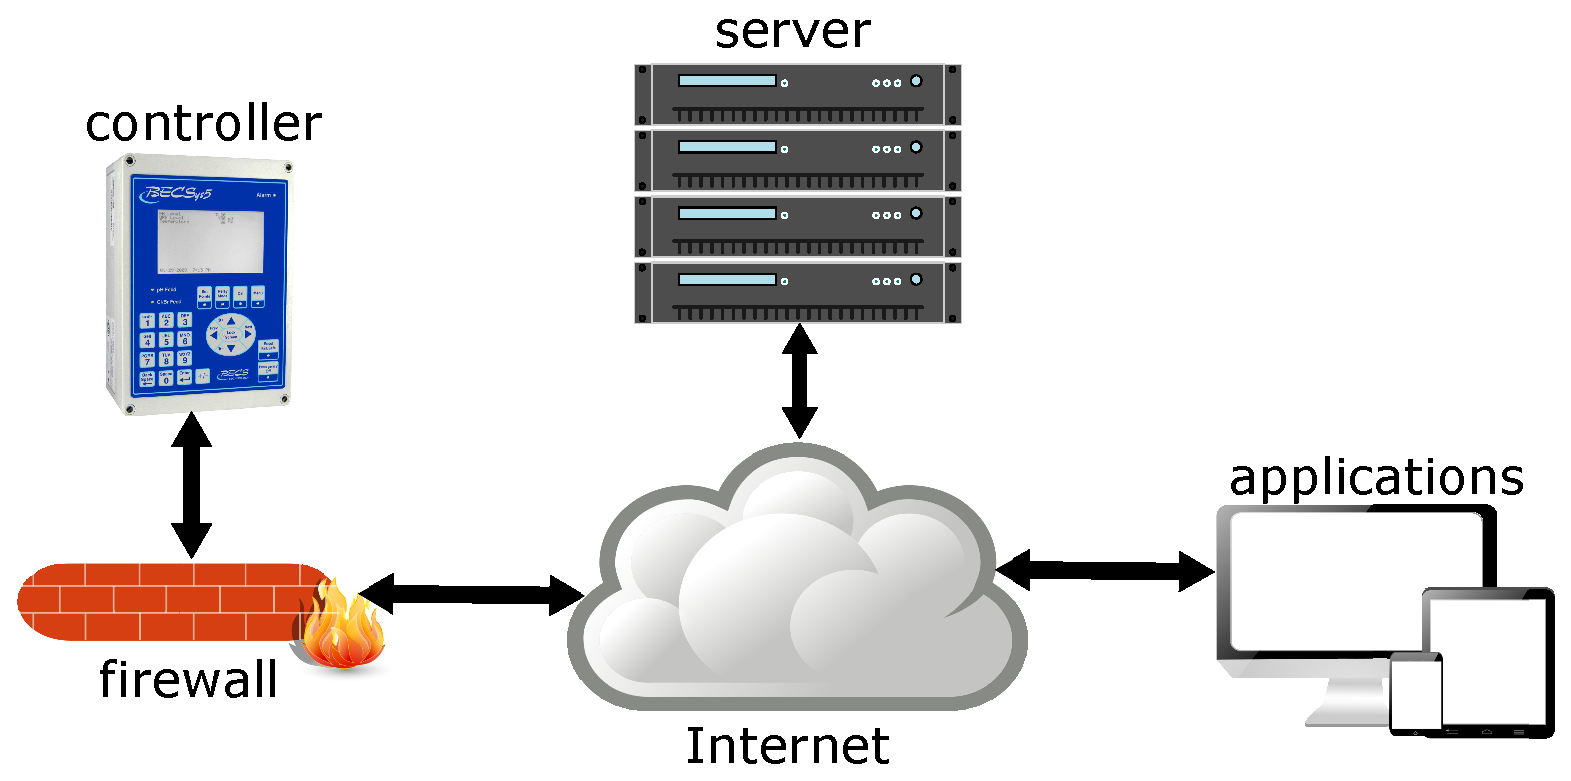
\includegraphics[width=\columnwidth]{EZConnect}
    \caption{EZConnect system diagram~\protect\cite{ezconnect}. The controller
opens a connection to the server in the cloud, which then facilitates communication with the controller by desktop programs or mobile apps.}
    \label{ezconnect}
\end{figure}

Remote capabilities include viewing of current status, downloading
of data logs, and configuration of the controller.
Figure~\ref{console} illustrates a realtime view of water chemistry
for a specific body of water
as remotely displayed on a PC screen.  Four readings are being shown:
pH (at\,7.1), ORP (at 750\,mV), temperature (at 83\,\degree F), and
free chlorine (at 1.0\,ppm).  Also indicated are the set points and
high and low alarm points for each reading as well as the control
outputs (in this example control is based on pH and ORP).
The two dials at the bottom show a pair of indices
(Langelier Saturation Index and Ryznar Stability Index)
which are indicators of the scaling properties of the water~\cite{mb88}.
The panel on the left allows the user to navigate to different
controllers (either at the same or a different physical location).
The tabs at the top allow the user to access a menu tree that
can examine and/or modify a multitude of parameters on the controller.

\begin{figure}[ht]
 \center
\includegraphics[width=0.9\columnwidth]{console}
    \caption{Console display of controller at remote location~\protect\cite{ccgss18}.}
    \label{console}
\end{figure}

Figure~\ref{graph} illustrates data logs collected over a 2 day period.
The same four readings are plotted on the top graph, and the bottom
graph gives indications of control actions, alarms, and other events.
In the top curve, one can readily see disturbances in the pH at noon
on both days.
The additional window on the right shows the instantaneous values
at the position of the cursor (the vertical line positioned
by the user at 9am on the first day).
As above, the leftmost panel supports navigation to different
controllers.

\begin{figure}[ht]
 \center
\includegraphics[width=1.0\columnwidth]{graph}
    \caption{Plot of controller data logs~\protect\cite{ccgss18}.}
    \label{graph}
\end{figure}

In addition to diagnosing the root causes of errors in the water
chemistry, the historical logs also enable the tracking of
parameter changes by operators as well as support the demonstration
and documentation of regulatory compliance.

The security of these controllers is
state-of-the-art~\cite{ezconnect,ccgss18}, with special attention given
to ease-of-use considerations, as there is ample evidence that
security measures that are difficult to implement are frequently
circumvented by users~\cite{gefen2000,hertzum2004,schneier16}.
Schneider~\cite{schneier16} cautions us all that security must
not rely on unreasonable expectations about the actions of users.
``We must stop trying to fix the user to achieve security.''
To be truly effective, any approach to security must be paired
with an approach to ease the burden on the user~\cite{gefen2000}.
Hertzum et al.~\cite{hertzum2004} assessed the intrinsic tensions between
security and ease of use in an e-banking context, and concluded
that ease of use limitations can directly contribute to decreased
security.

We must not sacrifice true security, however, in the name of ease
of use.  We need both, especially given the fact that
the security of IoT devices has been shown to be particularly
vulnerable, Cui and Stolfo~\cite{cs11} and Costin et al.~\cite{Costin2014}
have identified significant numbers of IoT devices
(over a million) with exposed vulnerabilities.

There has been significant work in the area of IoT and how it relates
to e-commerce.
Klock et al.~\cite{kpm11} describe the necessary infrastructure,
business possibilities, and barriers for e-commerce to thrive, particularly
as it relates to small- and medium-size enterprises.
Glova et al.~\cite{gsv14} analyze business models for the IoT environment,
reducing the business activity to its core elements, ``the value proposition,
distribution channels and the customers.''
Zhang and Wen~\cite{zw17} propose the use of blockchain technology in IoT
e-business,
and Xu~\cite{Xu14} reviews the development trends of IoT applications
in e-commerce.

Specific examples of IoT-based e-commerce include the following.
A decade ago,
Wamba et al.~\cite{wlbl08} assessed RFID technology's use in 
business-to-business e-commerce with a case study in the retail sector.
More recently,
Bi et al.~\cite{bxw14} described the impact of IoT on manufacturing, in
part driven by e-commerce.
Ruan and Shi~\cite{rs16} proposed an approach to monitoring the
freshness of fruit in-transit, and
Yu et al.~\cite{ywzh16} reviewed the state-of-the-art in
e-commerce logistics for supply chain management.
